\documentclass[conference]{IEEEtran}
\IEEEoverridecommandlockouts
\usepackage{cite}
\usepackage{amsmath,amssymb,amsfonts}
\usepackage{graphicx}
\usepackage{booktabs}
\usepackage{textcomp}
\usepackage{url}

% Federated results (Section VI-D), from results/experiment11_dtml/federated_final.csv (tag FEDc)
\newcommand{\FedMCC}{$0.040\pm0.022$}
\newcommand{\FedACC}{$0.523$}
\newcommand{\FedAUC}{$0.548$}
\newcommand{\FedWD}{$0.027$}

\begin{document}

\title{A Multi-Modal Graph Transformer for Federated Financial Forecasting:\\
Market Timing and Stock Selection on StockNet}

\author{\IEEEauthorblockN{Aditya M Hubli}
\IEEEauthorblockA{\textit{Dept. of Computer Science and Engineering} \\
\textit{PES University}\\
Bengaluru, India}
\and
\IEEEauthorblockN{Achintya N}
\IEEEauthorblockA{\textit{Dept. of Computer Science and Engineering} \\
\textit{PES University}\\
Bengaluru, India}
\and
\IEEEauthorblockN{Aditya Melkote}
\IEEEauthorblockA{\textit{Dept. of Computer Science and Engineering} \\
\textit{PES University}\\
Bengaluru, India}
\and
\IEEEauthorblockN{Aayush Prem}
\IEEEauthorblockA{\textit{Dept. of Computer Science and Engineering} \\
\textit{PES University}\\
Bengaluru, India}
}

\maketitle

\begin{abstract}
A next-day stock movement predictor can be right for two different reasons: it
can call the direction of the whole market on a given day, or it can rank stocks
correctly against each other. The standard pooled metric does not distinguish
the two. We present a multi-modal graph transformer (MMGT) for stock movement
prediction that is designed to do both. It extends a data-axis transformer, in
which every stock attends to every other stock and shares a market context, with
a per-stock profile built from volatility, SEC EDGAR fundamentals, tweet volume
and peer features derived from a stock graph. On the StockNet benchmark (87 US
stocks, 3{,}720 test predictions), MMGT reaches a Matthews correlation
coefficient (MCC) of $0.146\pm0.029$ over ten seeds, above every baseline we
trained on the identical split and above our own earlier tweet-count LSTM and
relational graph network ($p\le1.1\times10^{-5}$ in every comparison). A
within-day metric and a day-collapse control show where this comes from. Simple
per-stock models rank stocks but cannot time the market; the transformer
backbone times the market but loses the ability to rank stocks (within-day MCC
$0.008$, not distinguishable from zero); MMGT keeps the market timing and partly
restores stock selection (within-day MCC $0.023$, above the backbone on 8 of 10
seeds, $p=0.031$), and its multi-modal profile alone restores it to the level of
a per-stock LSTM. Hand-built graphs added to the attention layer bring no further
gain. Training with federated averaging across nine sector clients lowers pooled
MCC to $0.040$; under our fixed schedule the federated model barely improved
after its first round and behaves like a centralised model trained for one
epoch, so this gap reflects the training budget more than partitioning. The
model reported as ours was pre-registered before any test result was computed
and re-run with a corrected, leak-tested profile; every rung of the ablation is
reported.
\end{abstract}

\begin{IEEEkeywords}
stock movement prediction, graph transformer, multi-modal learning,
federated learning, StockNet, evaluation methodology
\end{IEEEkeywords}

% =====================================================================
\section{Introduction}

Financial markets respond to more than past prices: social media, company
filings and the behaviour of related firms all carry information about how a
stock may move. Since the StockNet benchmark of Xu and Cohen~\cite{xu2018stocknet}
paired price histories with tweets for 87 large US stocks, a long line of
models has combined these sources~\cite{feng2019advalstm,sawhney2020mansf,sawhney2021fast,yoo2021dtml},
and graph neural networks over inter-company relations have become a common
tool~\cite{chen2018gcn,feng2019rsr,cheng2022multimodality,wang2021review}.
Reported Matthews correlation coefficients (MCC) on StockNet range from close to
zero to about $0.19$~\cite{yoo2021dtml}, small numbers on a market that is close
to efficient~\cite{fama1970}.

These scores are computed by pooling every prediction of the test period, and a
pooled score can be earned in two quite different ways. A model can \emph{time
the market}, predicting correctly on which days most stocks will rise, or it can
\emph{select stocks}, ranking correctly which stocks will do better than others
on the same day. The first is rewarded heavily: on the StockNet test set, a
predictor that knows only each day's majority direction, and nothing about
individual stocks, reaches a pooled MCC of $0.625$. A gain in one ability is
therefore easily mistaken for a gain in the other.

We take this distinction as the organising question of the paper and build a
model meant to have both abilities. Our contributions are:
\begin{enumerate}
\item \textbf{A multi-modal graph transformer (MMGT).} We extend the data-axis
transformer DTML~\cite{yoo2021dtml}, in which every stock attends to every other
stock each day and all stocks share a market context, with a 47-dimensional
per-stock profile: realised volatility, SEC EDGAR fundamentals, tweet volume, and
peer features from a stock graph of sector, return-correlation and tweet
co-mention relations.
\item \textbf{Improvement over every baseline.} Over ten seeds MMGT reaches MCC
$0.146$, against $0.002$--$0.060$ for every baseline trained on the identical
split and for our own earlier models.
\item \textbf{Market timing and stock selection, separated.} Using a within-day
MCC and a day-collapse control, we show that simple per-stock models select
stocks but cannot time the market, that the transformer backbone times the market
but loses stock selection, and that MMGT keeps the timing while its multi-modal
profile restores stock selection.
\item \textbf{Graph and federation analysis.} Hand-built stock graphs help as a
source of peer features but not inside the attention layer. Federated
averaging~\cite{mcmahan2017fedavg} across sector clients lowers accuracy under a
fixed schedule, and a one-epoch centralised control shows that most of this gap
is under-training.
\item \textbf{A disciplined protocol.} Test data were locked during all tuning,
the model reported as ours was pre-registered~\cite{nosek2018} before any test
metric existed, and a feature leak found during review was fixed and verified
with a truncation test before the results reported here were computed.
\end{enumerate}

We do not claim a new state of the art: the attention backbone is DTML's, and our
reproduction of it scores below its published value.

% =====================================================================
\section{Related Work}

\textbf{Multi-modal stock movement prediction.} StockNet~\cite{xu2018stocknet}
introduced the benchmark used here and a variational model over tweets and
prices. Adv-ALSTM~\cite{feng2019advalstm} applied adversarial perturbations to
an attentive LSTM and released the preprocessed price features we use.
MAN-SF~\cite{sawhney2020mansf} fused tweets and prices bilinearly and applied
graph attention over company relations, and FAST~\cite{sawhney2021fast} modelled
the timing of news and tweets for trading. Recent work adds guided attention
over global and local news~\cite{ang2022guided}, causal treatment of
macroeconomic announcements~\cite{zhang2025camef}, sentiment-aware graph
learning~\cite{zhang2025gnnsentiment,nguyen2025dasf}, news embeddings~\cite{qayyum2025news},
hypergraphs over news events~\cite{harit2024breaking}, external knowledge
infusion~\cite{dukkipati2025predictive}, and explainable earnings
forecasts~\cite{li2024finreport}.

\textbf{Graphs and transformers for markets.} Relational models connect stocks
through industry or supply-chain links~\cite{chen2018gcn,feng2019rsr} or through
learned, time-varying relations~\cite{cheng2022multimodality,liu2025multimodal,hu2025differential,niu2025ngat},
with graph attention~\cite{velickovic2018gat} a common building block and hybrid
LSTM--graph and graph--transformer designs increasingly
used~\cite{sonani2025hybrid,zhu2025msgformer,kumar2024dynamic}; see~\cite{wang2021review}
for a review. Message passing on dense graphs is prone to over-smoothing, in which
node representations converge~\cite{li2018deeper}. Transformer-based
models~\cite{vaswani2017attention} avoid a fixed graph by letting stocks attend to
each other directly: DTML~\cite{yoo2021dtml} does so with a market context added
to each stock, and MASTER~\cite{li2024master} alternates within-stock and
across-stock attention under a market-guided gate.

\textbf{Federated and explainable financial learning.} Federated
averaging~\cite{mcmahan2017fedavg} trains a shared model without pooling raw
data, and has been applied to stock prediction~\cite{kumarappan2024federated,noseda2025federated},
multi-modal financial sentiment~\cite{zhong2025financial}, cross-border
financial graphs~\cite{tan2025graphprivacy}, and fraud detection, sometimes with
explainability~\cite{xia2025fingraphfl,aljunaid2025secure}.

\textbf{Evaluation.} We report MCC~\cite{matthews1975}, recommended over accuracy
and F1 for imbalanced binary problems~\cite{chicco2020mcc}, and follow work
showing that apparent architectural gains often vanish under controlled,
multi-seed re-evaluation~\cite{melis2018,henderson2018}.

% =====================================================================
\section{Data}

\textbf{Benchmark and splits.} We use StockNet~\cite{xu2018stocknet} in the
preprocessed form released with Adv-ALSTM~\cite{feng2019advalstm} and used by
DTML~\cite{yoo2021dtml}: 87 US stocks on a shared trading calendar from June 2013
to December 2015. A day is labelled \emph{up} if the stock's close-to-close return
exceeds $0.55\%$, \emph{down} if it is below $-0.5\%$, and is excluded otherwise.
The splits are chronological: training from 2 Jan.\ 2014 to 31 Jul.\ 2015 (398
trading days, 20{,}309 labelled samples), validation from 3 Aug.\ to 30 Sep.\ 2015
(42 days, 2{,}555 samples) and test from 1 Oct.\ to 31 Dec.\ 2015 (64 days,
3{,}720 samples, $51.3\%$ up). We verified that these 3{,}720 test samples match
those of our earlier experiments one-to-one, by stock, date and label, so every
result in this paper shares one test set.

\textbf{Price features.} Each stock-day carries the 11 features of
DTML~\cite{yoo2021dtml}: the open, high and low relative to the close; the daily
change of the close and adjusted close; and the ratio of the 5-, 10-, 15-, 20-,
25- and 30-day moving averages of the adjusted close to its current value. The
model sees the 10 trading days before the target date.

\textbf{Multi-modal profile.} For each stock and target day $t$ we build 47
features from information dated strictly before $t$, standardised with
training-split statistics and clipped to $\pm10$:
\begin{itemize}
\item \emph{Volatility (6):} realised volatility over the previous 5, 10 and 20
trading days, an exponentially weighted volatility ($\lambda=0.94$), and the
previous day's return and absolute return.
\item \emph{Fundamentals (20):} 13 SEC EDGAR quantities (revenue, net income,
assets, liabilities, equity, earnings per share, cash, three growth rates,
profit margin, debt-to-equity, return on assets) from the most recent record
before $t$, with seven missingness indicators.
\item \emph{Tweet volume (5):} log tweet counts on each of the four previous
trading days and their total.
\item \emph{Peer features (16):} derived from a daily stock graph that joins three
relations: same-sector membership (nine cliques, 381 edges); each stock's five
partners of highest absolute return correlation over the preceding 60 trading
days; and pairs of stocks mentioned together in a tweet over the preceding five
days. Over each stock's neighbours we compute the mean previous-day return,
absolute return and exponentially weighted volatility, the stock's own value
minus each mean, the logarithm of the number of neighbours, and a one-hot sector
code.
\end{itemize}

\textbf{Leakage control.} The close-to-close change on the target day itself
correlates $0.81$ with the label, while the same quantity on the last day the
model sees correlates $-0.006$, confirming the window alignment. For the profile
we use a stronger, mechanical test: for twelve target days spread over the three
splits, we rebuild the profile, and the correlation and co-mention edges that feed
its peer features, after deleting all data dated on or after the target day, and
require the result to be identical. It is, to the last bit.

% =====================================================================
\section{Model}

Fig.~\ref{fig:arch} summarises MMGT. White components follow DTML~\cite{yoo2021dtml};
shaded components are added in this work.

\begin{figure*}[t]
\centering
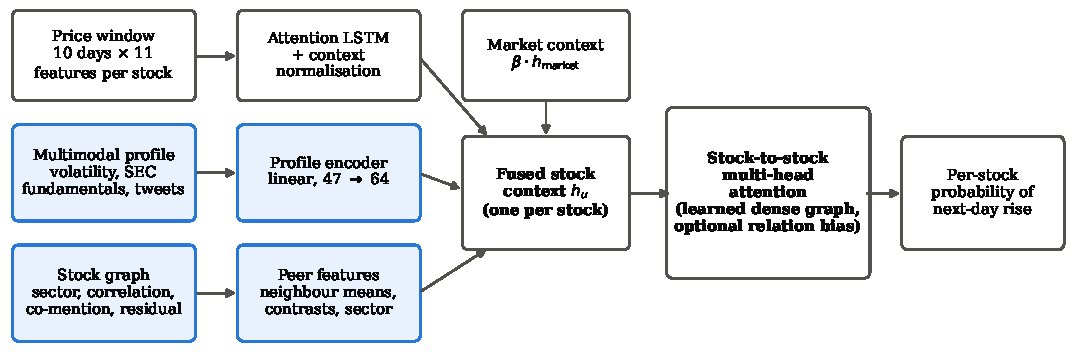
\includegraphics[width=\textwidth]{figures/architecture.pdf}
\caption{MMGT. Each stock's 10-day price window is summarised by an attention
LSTM, fused with an encoding of its multi-modal profile and a market context, and
passed through multi-head attention across all stocks of the day. Shaded
components are added in this work; white components follow DTML~\cite{yoo2021dtml}.}
\label{fig:arch}
\end{figure*}

\textbf{Temporal encoder.} For stock $u$, each day's feature vector is mapped by a
shared $\tanh$ layer and read by an LSTM~\cite{hochreiter1997lstm}. Rather than
keep only the last hidden state $h_T$, an attention step weights every hidden
state by its similarity to $h_T$ and sums them into a context $\tilde h_u$.
Context normalisation then standardises the contexts across all stocks of the
day and applies a learned per-stock scale and shift~\cite{yoo2021dtml}.

\textbf{Multi-modal fusion.} The 47-dimensional profile $p_u$ is mapped by a
linear layer to the context dimension and added:
$c_u = \mathrm{CN}(\tilde h_u) + W_p p_u$. The same attention LSTM applied to an
equal-weighted index of all stocks produces a market context $h_m$, giving
$h_u = c_u + \beta h_m$. Because $\beta h_m$ is identical for every stock on a
day, this term can only move all of a day's predictions together: it is the
model's market-timing pathway.

\textbf{Stock-to-stock attention.} The contexts of all stocks of the day form a
matrix $H$, to which multi-head self-attention~\cite{vaswani2017attention} is
applied along the stock axis, $\tilde H = \mathrm{softmax}(QK^\top/\sqrt{d})V$,
followed by $H' = \mathrm{LN}(\tanh(H + \tilde H + \mathrm{MLP}(H+\tilde H)))$.
This is attention over a complete graph of stocks whose edge weights are learned
for each day; the explicit stock graph enters through the peer features. As an
alternative we also inject the graph into this layer, either as a learned
per-head bias added to the attention scores of connected pairs for each of four
relations (sector, correlation, co-mention, and a market-residual correlation
graph), or as a mask that restricts attention to graph neighbours, as in graph
attention networks~\cite{velickovic2018gat}.

\textbf{Output and training.} A linear layer maps each row of $H'$ to the
probability of a rise. The loss is binary cross-entropy with an $L_2$ penalty on
the output layer only~\cite{yoo2021dtml}, plus a within-day pairwise ranking
term~\cite{burges2005ranknet}, $\frac{1}{|P||N|}\sum_{i\in P,j\in N}\log(1+e^{s_j-s_i})$,
over the stocks $P$ that rose and $N$ that fell on the day. Because this term is
unchanged when every score on a day shifts together, it can only be reduced by
ordering stocks correctly. We train with Adam~\cite{kingma2015adam} (learning
rate $10^{-4}$), one optimiser step per trading day, gradient-norm clipping at 1,
dropout $0.15$, hidden size 64, four heads and $\beta=1$, and select the
checkpoint with the highest validation MCC (patience 30, at most 200 epochs). All
training runs on CPU.

% =====================================================================
\section{Evaluation Protocol}

\textbf{Metrics.} The primary metric is MCC~\cite{matthews1975,chicco2020mcc} at a
0.5 threshold, with accuracy and AUC. Because the test set is $51.3\%$ up, an
always-up predictor reaches $51.3\%$ accuracy and MCC $0$.

\textbf{Market timing versus stock selection.} Two diagnostics separate the
abilities that pooled MCC mixes. \emph{Within-day MCC} thresholds each day's
predictions at that day's median and averages MCC over days; shifting every
stock's prediction on a day in the same direction earns nothing, so it measures
stock selection. The \emph{day-collapse} control replaces every prediction on a
day by that day's mean prediction and recomputes pooled MCC; whatever survives is
earned by calling the day's direction.

\textbf{Uncertainty.} Every model is trained with ten seeds unless stated and we
report mean $\pm$ standard deviation. Differences are tested with Welch's
$t$-test~\cite{welch1947}, paired by seed where both models share seeds. Single
runs are noisy because the market component of a 64-day test set has an
effective sample size near 64 rather than 3{,}720: a day-block
bootstrap~\cite{kunsch1989} gives per-run 95\% intervals of roughly $\pm0.14$
MCC, which is why we compare means over seeds.

\textbf{Discipline.} No configuration was selected on test data. A grid over
DTML's published search space (window $\{10,15\}$, $\beta\in\{0.01,0.1,1\}$,
hidden size $\{64,128\}$, learning rate $\{10^{-3},10^{-4}\}$; 48 runs) and all
later variants (39 runs) were evaluated on validation only. The test ladder,
including the model to be reported as ours (the configuration with the ranking
term), was committed to version control before its first test
run~\cite{nosek2018}. A review then found that the first version of the profile
was keyed to the target date in a table that contains only labelled rows, so the
presence of a row revealed whether that stock's move on the target day left the
buffer zone. We replaced it with the strictly-prior profile of Section~III,
verified by the truncation test, and re-ran every profile-based model with
unchanged configurations and seeds; only those re-run results are reported. The
reduced-feature and graph-attention variants were added after the main ladder,
each with its own pre-registered selection rule.

\textbf{Baselines.} Logistic regression and a two-layer MLP use the flattened
$10\times11$ price window; an LSTM and an attention LSTM (ALSTM~\cite{feng2019advalstm})
use MMGT's temporal encoder without stock attention or market context. Baselines
were not tuned, which favours our models. We also report two models from our own
earlier work on the same test samples: a tweet-count LSTM and a relational graph
convolutional network (RGCN) over sector and correlation edges. The RGCN's daily
graph contains only the stocks that carry a label on the target day, which
reveals which stocks moved outside the buffer zone; its score may therefore be
optimistic, which makes our comparison against it conservative. Our own models
include every stock with a complete input window, independent of the target day.

% =====================================================================
\section{Results}

\begin{table}[t]
\caption{Test results on StockNet (3{,}720 predictions). Mean $\pm$ s.d.\ over
ten seeds unless marked. WD: within-day MCC (stock selection).}
\label{tab:main}
\centering
\setlength{\tabcolsep}{3.2pt}
\begin{tabular}{lcccc}
\toprule
Model & MCC & Acc. & AUC & WD \\
\midrule
Logistic regression$^{\dagger}$ & $0.033$ & $0.517$ & $0.513$ & $0.004$ \\
LSTM & $0.022\pm0.021$ & $0.515$ & $0.528$ & $0.040$ \\
ALSTM & $0.045\pm0.038$ & $0.524$ & $0.533$ & $0.026$ \\
MLP & $0.057\pm0.020$ & $0.528$ & $0.536$ & $0.000$ \\
Tweet-count LSTM$^{\ddagger}$ & $0.002\pm0.011$ & -- & -- & -- \\
RGCN graph$^{\ddagger}$ & $0.060\pm0.018$ & -- & -- & $0.005$ \\
\midrule
DTML backbone, reproduced & $0.139\pm0.049$ & $0.558$ & $0.593$ & $0.008$ \\
\textbf{MMGT (ours)} & $\mathbf{0.146\pm0.029}$ & $\mathbf{0.570}$ & $\mathbf{0.602}$ & $0.023$ \\
MMGT, federated$^{\S}$ & \FedMCC & \FedACC & \FedAUC & \FedWD \\
\bottomrule
\multicolumn{5}{l}{\footnotesize $^{\dagger}$Deterministic, one run. $^{\ddagger}$Our earlier work, five seeds;}\\
\multicolumn{5}{l}{\footnotesize \phantom{$^{\ddagger}$}the RGCN score may be optimistic (Section V).}\\
\multicolumn{5}{l}{\footnotesize $^{\S}$Without the ranking term; five seeds, FedAvg over nine sector}\\
\multicolumn{5}{l}{\footnotesize \phantom{$^{\S}$}clients; largely under-trained (Section VI-D).}\\
\end{tabular}
\end{table}

\begin{figure}[t]
\centering
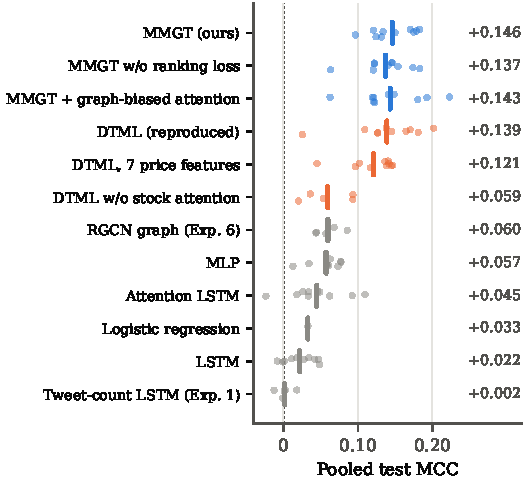
\includegraphics[width=\columnwidth]{figures/seeds.pdf}
\caption{Pooled test MCC of every seed (dots) and the mean (bar). Blue: MMGT and
its variants; orange: the DTML backbone and its ablations; grey: baselines.}
\label{fig:seeds}
\end{figure}

\subsection{MMGT outperforms every baseline}

Table~\ref{tab:main} and Fig.~\ref{fig:seeds} give the main results. MMGT reaches
MCC $0.146\pm0.029$, accuracy $57.0\%$ and AUC $0.602$. Every baseline trained on
the identical split scores between $0.022$ and $0.057$, and our earlier
tweet-count LSTM and RGCN score $0.002$ and $0.060$. The improvement over each is
significant: against the MLP $p=6.6\times10^{-7}$, the ALSTM $p=3.4\times10^{-6}$,
the LSTM $p=6.9\times10^{-9}$, logistic regression $p=6.6\times10^{-7}$, the RGCN
$p=1.1\times10^{-5}$ and the tweet-count LSTM $p=6.2\times10^{-9}$; all six remain
significant after Bonferroni correction. Every one of the ten MMGT seeds, the
lowest at $0.097$, lies above the best baseline mean.

The reproduced DTML backbone scores $0.139\pm0.049$, not significantly below MMGT
in pooled MCC (paired $p=0.65$). Our reproduction falls short of the $0.191$
reported for DTML~\cite{yoo2021dtml}; we approximate its S\&P~500 market index by
an equal-weighted index of the 87 stocks, and seeds and selection details differ.
What separates MMGT from the backbone is not the pooled score but where it comes
from.

\subsection{Market timing and stock selection}

\begin{table}[t]
\caption{Where the score comes from (test, ten seeds). Pooled MCC rewards both
abilities; within-day MCC only stock selection; day-collapse MCC only market timing.}
\label{tab:timing}
\centering
\setlength{\tabcolsep}{3.5pt}
\begin{tabular}{lccc}
\toprule
Model & Pooled & Within-day & Day-collapse \\
\midrule
LSTM (per-stock) & $0.022$ & $0.040\pm0.014$ & $0.006$ \\
DTML backbone & $0.139$ & $0.008\pm0.014$ & $0.130$ \\
\textbf{MMGT (ours)} & $0.146$ & $0.023\pm0.018$ & $0.219$ \\
\midrule
Market-direction oracle & $0.625$ & $0$ & $0.625$ \\
\bottomrule
\end{tabular}
\end{table}

Table~\ref{tab:timing} decomposes the scores. The per-stock LSTM selects stocks:
its within-day MCC, $0.040$, is clearly above zero ($p=1.1\times10^{-5}$). It
cannot time the market, so its day-collapse MCC is $0.006$ and its pooled score
low. The DTML backbone is the reverse. Collapsing each day to its mean prediction
keeps almost all of its pooled score ($0.130$ of $0.139$), while its within-day
MCC, $0.008$, is not distinguishable from zero ($p=0.12$): the shared market
context moves all of a day's predictions together, and the model has traded stock
selection for market timing.

MMGT keeps the market timing and recovers part of the stock selection. Its
day-collapse MCC, $0.219$, shows strong market timing, and its within-day MCC,
$0.023$, is above zero ($p=0.003$) and above the backbone's on 8 of 10 seeds
(paired $p=0.031$), though still below the per-stock LSTM's $0.040$ ($p=0.031$).
The ablations below attribute the recovered stock selection to the multi-modal
profile.

\subsection{Ablations}

\begin{table}[t]
\caption{Ablations (test). One change per row; seeds in parentheses.}
\label{tab:ablation}
\centering
\setlength{\tabcolsep}{4pt}
\begin{tabular}{lcc}
\toprule
Variant & Pooled MCC & Within-day \\
\midrule
DTML backbone (10) & $0.139\pm0.049$ & $0.008$ \\
\quad without stock attention (5) & $0.059\pm0.033$ & $0.022$ \\
\quad 7 of 11 price features (10) & $0.121\pm0.032$ & $-0.001$ \\
\quad + multi-modal profile (10) & $0.137\pm0.033$ & $0.031$ \\
\quad + profile + graph-biased attention (10) & $0.143\pm0.046$ & $0.028$ \\
\midrule
MMGT = backbone + profile + ranking term (10) & $0.146\pm0.029$ & $0.023$ \\
\quad without market context (5) & $0.078\pm0.040$ & $0.024$ \\
\bottomrule
\end{tabular}
\end{table}

Table~\ref{tab:ablation} isolates each component.

\textbf{The profile restores stock selection.} Adding the multi-modal profile to
the backbone raises within-day MCC from $0.008$ to $0.031$, higher on 8 of 10
seeds (paired $p=0.011$) and indistinguishable from the per-stock LSTM's $0.040$
($p=0.30$), without changing pooled MCC ($0.137$ against $0.139$, $p=0.93$). The
ranking term on top of it changes neither metric significantly
(pooled $0.146$ against $0.137$, $p=0.46$; within-day $0.023$ against $0.031$,
$p=0.35$); it is retained because it is part of the pre-registered model.

\textbf{Stock-to-stock attention and the market context carry the pooled score.}
Removing stock attention from the backbone lowers pooled MCC from $0.130$ to
$0.059$ on the same five seeds (lower on 4 of 5, paired $p=0.048$). Removing the
market context from MMGT lowers it from $0.131$ to $0.078$ on the same five seeds
(lower on 4 of 5, $p=0.12$), while within-day MCC is unchanged, as expected for
the market-timing pathway.

\textbf{Feature count matters little.} Keeping only the daily return and the six
moving-average ratios, 7 of 11 price features, gives $0.121$, not significantly
below the full set (paired $p=0.21$). On validation, a single feature, the daily
return, already reached MCC $0.188$.

\textbf{A hand-built graph does not improve learned attention.} Adding learned
relation biases for four graph relations to the attention scores gives $0.143$,
not different from the same model without them (paired $p=0.45$). Restricting
attention to graph neighbours, the graph-attention design, was clearly worse on
validation (MCC $0.223$ against $0.279$) and by our pre-registered rule was not
taken to test. The stock graph is useful as a source of peer features, but the
model learns more useful stock-to-stock weights than the fixed relations supply.

\subsection{Federated training}

We trained the profile model (without the ranking term) with federated
averaging~\cite{mcmahan2017fedavg} across nine sector clients, each holding 7--10
stocks. In each round every client trains one local epoch on its own stocks only,
with attention and loss restricted to them, and the server averages the client
weights in proportion to their training samples; the global model is selected on
validation MCC over at most 40 rounds (patience 10).

\begin{table}[t]
\caption{Federated versus centralised training of the profile model (test, the
same five seeds). The one-epoch row is a centralised control for the short
federated schedule.}
\label{tab:fed}
\centering
\setlength{\tabcolsep}{4pt}
\begin{tabular}{lccc}
\toprule
Training & Pooled & Within-day & Day-collapse \\
\midrule
Centralised, fully trained & $0.115$ & $0.024$ & $0.103$ \\
Federated (FedAvg) & $0.040$ & $0.027$ & $-0.024$ \\
Centralised, one epoch & $0.053$ & $0.016$ & $0.035$ \\
\bottomrule
\end{tabular}
\end{table}

Table~\ref{tab:fed} gives the result. Each client trains on its own sector's
stocks and labels only, while the market index and the peer features are built
from public prices of all stocks, so what a client lacks is the other sectors'
stocks in the attention layer and their labels. Federation lowers pooled MCC from
$0.115$ to $0.040$, lower on all five seeds ($p=0.017$). Through the same
decomposition, the loss is in market timing (day-collapse $0.103$ against
$-0.024$, $p=0.003$) while within-day MCC is unchanged ($0.027$ against $0.024$,
$p=0.80$) and still above zero ($p=0.018$).

This pattern cannot be attributed to partitioning. In four of five seeds the best
global model came from the first round, and a centralised model stopped after one
epoch looks much the same: pooled $0.053$, day-collapse $0.035$, within-day
$0.016$. Under the fixed schedule, then, most of the federated gap is
under-training, and measuring the cost of partitioning itself requires a longer
schedule. Because every input here is public market data, the experiment does not
provide a privacy guarantee; no secure aggregation or differential privacy is
applied.

% =====================================================================
\section{Discussion}

\textbf{What the pooled score hides.} On this test set a market-direction oracle
scores $0.625$ and a per-stock LSTM with genuine stock-selection skill scores
$0.022$, so pooled MCC ranks models largely by their market timing. Our backbone
illustrates the consequence: it outscores every baseline while having lost the
stock-selection skill the baselines have. Models with a shared market
signal~\cite{yoo2021dtml,li2024master} deserve the same scrutiny. Reporting
within-day MCC and a day-collapse score next to pooled MCC costs nothing and makes
the distinction visible.

\textbf{Why the profile helps.} The market context adds the same vector to every
stock, which pushes the attention layer toward day-level signals. The profile adds
stock-specific information the price window lacks: how volatile a stock has been,
its fundamentals, its attention on social media, and how it compares with its
graph neighbours. This information differs across stocks on the same day, which
is exactly what within-day ranking needs.

\textbf{Limitations.} We study one benchmark of 87 large US stocks over
2014--2015 with a 64-day test period, so the market component of every score rests
on few independent days. The attention backbone is DTML's, and our equal-weighted
market index approximates the S\&P~500 it used. Comparisons among our own model
variants are not corrected for multiple testing; the comparisons against
baselines survive a Bonferroni correction. Baselines were not tuned. Federation
is simulated on a single machine with an untuned schedule. We did not evaluate
explanation methods: attention maps over stocks are available from the model, but
without validation we do not interpret them.

% =====================================================================
\section{Conclusion}

MMGT, a multi-modal graph transformer that adds volatility, fundamentals, tweet
volume and graph-derived peer features to a data-axis attention backbone, reaches
MCC $0.146$ on StockNet over ten seeds and outperforms every baseline we trained
on the same split as well as our own earlier models. Separating market timing from
stock selection explains the result: per-stock models select stocks but cannot
time the market, the attention backbone times the market but loses stock
selection, and MMGT keeps the timing while its multi-modal profile restores stock
selection. Learned attention across stocks was more useful than any fixed graph we
supplied. Federated training across sector clients scored lower under a fixed
schedule, mostly because it stopped near its first round; isolating the cost of
partitioning is left to longer schedules. We recommend that work on this benchmark report within-day and
day-collapse scores alongside pooled MCC, use multiple seeds, and select models
on validation data only.

\section*{Acknowledgment}

We thank our guide, Dr.~Mamatha H R, Department of Computer Science and
Engineering, PES University, for guidance throughout this project
(PW26\_MHR\_03).

\section*{Reproducibility}

Code, the pre-registration file with its commit history, per-seed results, the
leakage test, and the scripts that produce every table and figure are available in
the project repository.

\bibliographystyle{IEEEtran}
\bibliography{refs}

\end{document}
